
\documentclass[12pt]{beamer}
\usepackage{xcolor}
\usepackage{pgf,pgfarrows,pgfnodes,pgfautomata,pgfheaps,pgfshade}
\usetheme{Air}

\DeclareMathOperator*{\argmax}{arg\,max}

\title[CSC349A Numerical Analysis]{CSC349A Numerical Analysis}


\logo{\pgfputat{\pgfxy(-0.5,7.5)}{\pgfbox[center,base]{
\includegraphics[width=1.0cm]{figures/uvic}}}}  
\beamertemplatenavigationsymbolsempty

    \defbeamertemplate{footline}{author and page number}{%
      \usebeamercolor[fg]{page number in head/foot}%
      \usebeamerfont{page number in head/foot}%
      \hspace{1em}\insertshortauthor\hfill%
      \insertpagenumber\,/\,\insertpresentationendpage\kern1em\vskip2pt%
    }
    \setbeamertemplate{footline}[author and page number]{}



\subtitle[Leture 1]{Lecture 1}
\date[2025]{2025}
\author[G. Tzanetakis]{George Tzanetakis}
\institute[University of Victoria]{University of Victoria}
%\logo{\includegraphics[scale=.25]{unilogo.pdf}}
\begin{document}
\frame{\maketitle} % <-- generate frame with title


\AtBeginSection[]
{
\begin{frame}<beamer>[allowframebreaks]{Table of Contents}
\tableofcontents[currentsection,currentsubsection, 
    hideothersubsections, 
    sectionstyle=show/shaded,
]
\end{frame}
}


\section{Logistics} 

\begin{frame}{Course Information} 
\begin{itemize} 
\item{Course outline: \url{https://course-outlines.uvic.ca/ban/course-outlines/public-outline?banner_term=202509&subject=CSC&course_number=349A}}
\item{{\bf Optional} Textbook: Numerical Methods for Engineers  (8th edition), S.C. Chapra and R.P. Canale,McGraw-Hill, ISBN: 978-0-07-3397924 }
\item{The new edition of this book is available as an e-book.}
\item{ MATLAB - \url{https://matlab.engr.uvic.ca/student/}}
\item{ Python - \url{https://www.spyder-ide.org/}}
\end{itemize} 
\end{frame} 

\begin{frame}{Grading} 
\begin{itemize} 
\item{6 assignments worth $30\%$ of final grade}
\begin{itemize} 
\item{No extensions unless the whole class gets one}
\end{itemize}
\item{2 Midterms $30\%$ and Final Exam $40\%$.}
\item{If you miss a midterm due to illness, there will be an alternative weighting}
\begin{itemize} 
\item{1 Midterm $20\%$ and Final Exam $60\%$}
\item{Note - You can't miss two midterms}
\end{itemize}
\item{If you miss the final due to illness, apply for a Deferal}
\begin{itemize} 
\item{Note - will not be granted if you also missed a midterm}
\end{itemize} 
\item{You will be marked for both correctness and logic}
\item{Early errors are worse than late errors}
\item{Errors propogate, you do not get credit for wrong answers}
\end{itemize} 
\end{frame} 

\begin{frame}{Attendance} 
\begin{itemize}
\item{Not compulsory - you are adults} 
\item{DO NOT email me when you will miss a lecture} 
\item{Handouts and associated coursepack} 
\item{Lecture notes, and slides}
\item{I will NOT be recording or streaming the lectures}
\item{{\bf USE BRIGHTSPACE:} \url{https://bright.uvic.ca/d2l/home/314357}}
\end{itemize}
\end{frame} 

\begin{frame}{Large scale challenges} 
\begin{itemize} 
\item{~200 students} 
\item{{\bf USE BRIGHTSPACE and PRAIRIELEARN}} 
\item{If you e-mail me, be precise - always CSC349A in subject line, mention assignment etc} 
\item{Less flexibility and feedback on assignments}
\end{itemize}
\end{frame} 

\begin{frame}{Assignments}
\begin{itemize} 
\item{Online through {\bf PRAIRIELEARN}}
\item{Answers to be separated by question}
\item{Any recycling of answers from previous 
years automatically zero grade on assignment and AIC case brought forward} 
\item{{\bf NO LATE SUBMISSIONS}}
\end{itemize}

\end{frame}

\begin{frame}{Academic Integrity}
\begin{itemize} 
\item{The CSC department has an Academic Integrity Committee (AIC)}
\item{Any violations of Academic Integrity will be forwarded to the AIC}
\item{UVic has strict policies against AI violations}
\begin{itemize}
\item{\url{https://www.uvic.ca/students/academics/academic-integrity/index.php}}
\end{itemize}
\item{Once a violation has be sent to the committee it is out of my hands}
\end{itemize}
\end{frame}

\begin{frame}{Highlights of UVic AI Policy}
\begin{itemize} 
\item{Single or multiple instances of plagiarism should result in a failing grade for the work.}
\item{A largely or fully plagiarized piece of work should result in a grade of F for the course.}
\item{Isolated instances of copying during an exam should result in a grade of zero for the exam.}
\item{Systematic copying during an exam should result in a grade of F for the course.}
\item{Any instance of any of the violations committed by a repeat offender, should result in the student being placed on disciplinary probation.}
\item{A letter of reprimand will be sent to the student and a copy shall be included in the record maintained by the Office of the Registrar.}
\end{itemize}
\end{frame}


\section{What is numerical analysis?} 

\begin{frame}{Definition}


\begin{block}{Numerical analysis} 
{\bf Numerical analysis} is concerned with accurate, efficient approximations
of solutions to problems of continuous mathematics.
\end{block}
\end{frame} 

\begin{frame}{Rounding Errors} 
\begin{block}{}
Real and complex numbers can not be represented exactly on computers 
therefore they are always {\bf approximated}. This approximation introduces 
errors which, even though typically small, can have a significant effect 
in the accuracy of numerical computations especially when these 
computations involve lots of arithmetic operations. 
\end{block}

\begin{block}{}
Numerical analysis investigates the {\bf stability} and {\bf accuracy} of
algorithms on these rounding errors. 
\end{block}
\end{frame}


\begin{frame}{Truncation Errors} 

\begin{block}{}
Most continuous mathematics algorithms {\bf cannot be solved by finite algorithms}. 
This is true even if we could somehow work with exact arithmetic. This is true for many problems of interest including zero finding, differential equations, and optimization. 
\end{block}

\begin{block}{}
Rapid {\bf convergence of approximations} is the primary challenge that has been met 
successfully by numerical analysis.
\end{block}{}
\end{frame} 






\begin{frame}{Continuous mathematics applications} 
\begin{itemize} 
\item{Physics engines in computer games - Angry birds}
\item{Simulating wind turbulance - wing design}
\item{Filter design - audio effects} 
\item{Non-linear least squares - 3D models from photographs}
\item{Optimization - a lot of data mining, machine learning}
\item{Matrix computations - 3D graphics for games} 
\item{Differential equations - simulation in ECE, MEC}
\item{Study of errors - major disasters due to numerical errors} 
\end{itemize} 
\end{frame} 



\begin{frame}{Historical Origins of Numerical Analysis} 

\begin{itemize} 
\item{Computers were people before they were machines}
\item{World War II was the catalyst for the development of computers} 
\item{Code breaking was the original discrete mathematics killer (literally) 
app}
\item{Computation of ballistic tables and atomic bomb simulations were the 
original continuous mathematics killer (literally) apps}
\end{itemize} 

\end{frame} 


\begin{frame}{Importance in science and engineering} 
\begin{itemize}
\item{Powerful problem solving tools that can handle large amounts of data, non-linearities and complex geometries that {\bf cannot} be solved by any other means} 
\vspace{\baselineskip}
\item{Under the hood knowledge of packaged software} 
\vspace{\baselineskip}
\item{Not all real-world problems can be solved with packaged software} 
\end{itemize} 
\end{frame} 

\begin{frame}{Book overview} 
\begin{itemize}
\item{8 parts and 32 chapters} 
\item{Each part begins with a Preface motivating each problem 
and some background mathematics} 
\item{Part 1: Modelling, computers and error analysis}
\item{Part 2: Roots of equations}
\item{Part 3: Linear algebraic equations}
\item{Part 5: Curve fitting}
\item{Part 6: Differentiation \& integration}
\item{Part 7: Ordinary differential equations}
\item{Each part ends with Case Studies from Engineering to highlight the applications}
\end{itemize} 
\end{frame} 

\section{A motivating example} 


\begin{frame}{Mathematical Models}
These equations are typical of mathematical models of the physical
world: 

\begin{itemize} 
\item{Describes a natural process in mathematical terms}
\item{It represents an idealization and simplification of reality} 
\item{It yields reproducible results and can be used for predictive
    purposes} 
\end{itemize} 
\end{frame}


\begin{frame}{A motivating example}
Determine the terminal veloctiy of a free-falling body (a parachutist)
near the earth's surface by using Newton's second law of motion and solving a differential equation by, 
(a) analytical methods, then (b) numerical methods, and 
(c) compare.

\vspace{2 in}

\end{frame}


\begin{frame}{A motivating example continued}
Using Newton's second law in our parachutist example, with downward pull of gravity given by $mg$, where $m$ is mass and $g$ is the gravity constant, and the upward force of air resistance given by $-cv$, where $c$ is the drag coefficient and $v$ is the velocity, we derive the following model to express the problem.

\[
\frac{dv}{dt}=g-\frac{c}{m}v
\]

Here, we have a differential equation in terms of the rate of change of velocity over time, given by $t$.
\vspace{2 in}
\end{frame}

\begin{frame}{Analytical solution} 
It is possible to get an
analytic solution to this differential equation using calculus. If the 
object is initially at rest i.e $v = 0$ at time $t = 0$ then: 

\begin{equation} 
v(t) = \frac{gm}{c} (1 - e^{-\frac{ct}{m}})
\end{equation} 


This analytical solution can be used directly to solve
problems. 

\vspace{0.25 in}

For example, let  $m=68.1 kg$ , $g=9.81 m/s^2$, and $c=12.5 kg/s$.

\end{frame} 

\begin{frame}{Analytical solution - Example 1.1}

For example a parachutist of mass $68.1 kg$ jumps out of a stationary hot
air balloon. The drag coefficient is equal to $12.5 kg/sec$. 

Inserting the parameters into the equation we get: 

\begin{table} 
\begin{tabular}{|c|c|} 
\hline
{\bf t}    & {\bf v} \\ 
\hline 
0   &  0.0 \\ 
2   &  16.40 \\ 
4   &  27.77 \\ 
6   &  35.68  \\
..   &  ..  \\
$\infty$ & 53.44 \\ 
\hline
\end{tabular}
\end{table} 
  

Thus the {\it terminal velocity} is $53.44 m/sec$ for this example. 
 
\end{frame} 


\begin{frame}{Numerical solution}
Numerical approach (in constrast to analytical) for solving this
mathematical model. Not exact but we can get arbitrarily close. Why numerical methods (NM) ? 
\begin{itemize} 
\item{NM can be applied to functions for which we can
    not easily find an analytical solution through Calculus} 
\item{As any equation is to some degree an approximation of reality
  and therefore errors are inevitable it is possible depending on the
  application that the errors introduced by NM are neglible in the
  context of the desired application}
\item{It's extremely simple to write a computer program to do the job 
for us although the number of mathematical operations involved is much
larger than the analytical solution} 
\end{itemize} 

\end{frame}

\begin{frame}{Numerical Solution}
\begin{itemize} 

\item{The idea is rather simple. We will approximate the derivative of the
function by a ``finite divided difference'' effectively discretizing
time.}
\vspace{0.1 in}
\item{If we denote the discrete time steps we take as $t_{i}$ (we can decide what 
sampling rate is appropriate depending on the application) then we can
approximate the derivative at time $t_{i}$ as follows:
\[
\frac{dv}{dt} \approx \frac{v(t_{i+1})-v(t_i)}{t_{i+1}-t_i}
\]
}
\end{itemize} 

\end{frame} 

\begin{frame}{Numerical Solution continued}
So, if we substitute our derivative approximation into our model differential equation, we can derive an approximation formula for the velcoity at time $t_{i+1}$ given the velocity at time $t_i$, as follows.

\[
v(t_{i+1}) \approx v(t_i)+\left[g-\frac{c}{m}v(t_i)\right](t_{i+1}-t_i)
\]

\end{frame} 

\begin{frame}{Numerical iteration}
\begin{itemize} 
\item{Notice that this equation gives us a way to compute the velocity value
at time $t_{i+1}$ based on the previous value of the velocity.}
\vspace{\baselineskip}
\item{This approach is called Euler's method can be verbally expressed as: 
{\it New value = old value + slope x step size}.}

\end{itemize}
\end{frame}


\begin{frame}{Numerical solution - Example 1.2}
\begin{itemize} 
\item{For example we can
use it to compute the velocity values with a step size of $2$
seconds.}

\item{At the start of the computation we use an initial velocity value
$v_{0} = 0$ for $t_{0} = 0$ plug the numbers into the equation 
and get the value of $v_{1}$. Then we can use the value at $v_{1}$ to 
compute the value at $v_{2}$ and so forth.
}
\end{itemize}

\[
v(t_1) \approx v(t_0)+\left[g-\frac{c}{m}v(t_0)\right](t_1-t_0)
\]

\end{frame}

\begin{frame}{Numerical solution - Example 1.2}
\begin{itemize} 
\item{For example we can
use it to compute the velocity values with a step size of $2$
seconds.}

\item{At the start of the computation we use an initial velocity value
$v_{0} = 0$ for $t_{0} = 0$ plug the numbers into the equation 
and get the value of $v_{1}$. Then we can use the value at $v_{1}$ to 
compute the value at $v_{2}$ and so forth. }
\end{itemize}
\begin{table} 
\begin{tabular}{|c|c|} 
\hline
{\bf t}    & {\bf v} \\ 
\hline 
0   &  0.0 \\ 
2   &  19.62 \\ 
4   &  32.04 \\ 
6   &  39.90  \\
..   &  ..  \\
$\infty$ & 53.44 \\ 
\hline
\end{tabular}
\end{table} 
\end{frame}

\begin{frame}{Comparison}
\begin{figure}[ht]
  \centering
  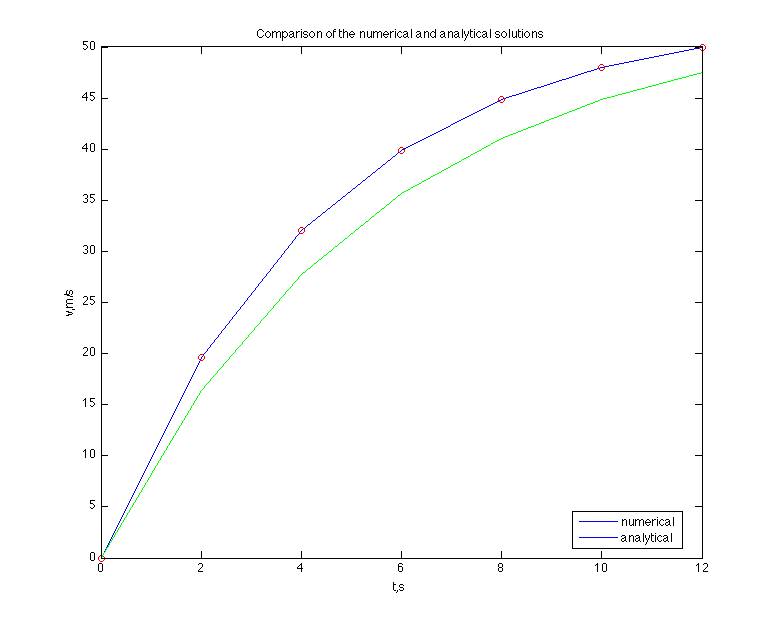
\includegraphics[scale=0.35]{comparison_numerical_analytical}
  \caption{Comparison of numerical and analytical solution}
  \label{fig:comparison}
\end{figure}





\end{frame}


\begin{frame}{Comparison of numeric and analytic solution}
Figure ~\ref{fig:comparison} shows a plot comparing the results of the
numerical approximation using Euler's method and the exact analytical
solution. In engineering there is frequently a tradeoff between
accuracy and computational resources. 
\end{frame} 

\begin{frame}{Euler Method} 
The Euler method and more generally numerical methods allow you to
control that tradeoff for example by adjusting the step size
appropriately for the program at hand. There are several questions one
could ask at this point that we will be exploring in the rest of the
course. For example can we show that the error between the exact
solution and the numerical approximate solution will always decrease
with smaller step size? Can we compare how long different approaches
to approximating the derivative of a function take? Are there any
functions for which this would not work? Could we reduce the number
of multiplication/additions needed to perform each step of the
iteration?

\end{frame}

\end{document}

